This project investigates whether biologically inspired spiking neural network can be used to recognise and track simple shapes moving in a video stream in real time. The network developed for this project currently recognised squares and diamonds in synthetic videos. 

In this chapter a brief introduction on the functioning of biological neurons and the technologies used in order to simulate them will be presented. A quick discussion on the motivation and previous work in the area will also be provided. 

All of the following tools and technologies had been selected in order to develop a project with as many similarities as possible to the functioning of a biological brain. 


\section{Neuron}
Neurons are highly specialised cells found in the nervous system designed to generate and transmit electrical signals to other cells. Many different kinds of neurons exist \cite{Llinas:2008}, each with different morphology, but a typical neuron can be divided in the three parts shown in \cref{fig:neuron_morphology} \textbf{A}:
\begin{itemize}
    \item Soma: a usually compact area which represents the body of the neuron and which contains the cell nucleus.
    \item Dendrites: tree-like extensions of the soma membrane which acts as the ``input'' pole to the neuron.
    \item Axons: a cable-like structure that acts as the ``output'' pole of the neuron and propagate neuronal output to other cells.
\end{itemize}
The axon of a \textit{presynaptic cell} makes contact with the dendrite of a \textit{postsynaptic cell} at a site called synapse \cite{Gerstner:2014}, highlighted in \cref{fig:neuron_morphology} \textbf{B}.

\begin{figure}[ht]
\centering
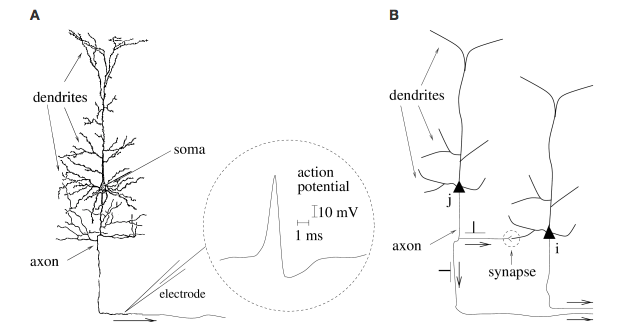
\includegraphics[scale=0.6]{images/context/neuron.png}
\caption[Neuron Morphology]{\textbf{A}. Cortical pyramidal cell with its soma, axon and dendrites highlighted. \textbf{B}. Signal transmission from neuron $j$ (presynaptic cell) to neuron $i$ (postsynaptic cell). Reproduced from \cite{Gerstner:2014}.}
\label{fig:neuron_morphology}
\end{figure}

A neuron spikes when the current input carried by the dendrites exceeds a certain threshold. The biochemical details of this process are not relevant for this project and the variety in electrophysiological properties of neurons \cite{Llinas:2008} leads to necessary simplification in order to simulate them. The signals emitted by neurons are called action potentials or spikes, and an approximate form is shown in the circled area of  \cref{fig:neuron_morphology}. A key property of action potential is that the form does not carry any information, information is actually carried by the number of action potentials and their timings \cite{Gerstner:2014}. After each spike the neuron enters a state called refractory period, in which it is impossible for it to spike again.  

Several mathematical models are available in order to simulate neurons, the one used in this project is a leaky integrate-and-fire (LIF) neuron model. 

% TODO insert maths details of LIF model

\subsection{Spiking Neural Networks}
Spiking neural networks are artificial neural networks which are closer to biology than the one commonly used nowadays for machine learning tasks. In spiking neural networks the concept of time is introduced and the communication between neurons relies exclusively on discrete spikes, the ones described in the previous section, instead of continuous values. 

The field of spiking neural networks is still in its infancy and lacks an effective supervised method for training, the equivalent of backpropagation for artificial neural network.


\section{SpiNNaker}
In order to handle the obvious complexity of neural simulation two approaches are possible. The first one is to use supercomputer built for general purpose task like in the case of the Blue Brain project which uses IBM's Blue Gene supercomputers \cite{Markram2006}. The second approach is to employ neuromorphic systems. These systems are designed around the idea that small computing elements (the ``neurons'') perform computation in a highly distributed manner in ways that mimic biological brains \cite{Furber2016}. Several of these systems have been developed recently, for example IBM TrueNorth, Stanford Neurogrid and University of Manchester SpiNNaker, which will be the system used for this project.

SpiNNaker is a massively-parallel multi-core computing system designed for large scale brain simulations running in biological real time. The system had been designed focusing on scalability, in order to model the very large number of components in a biological brain, and energy efficiency.

\begin{figure}[ht]
\centering
\begin{subfigure}{0.45\textwidth}
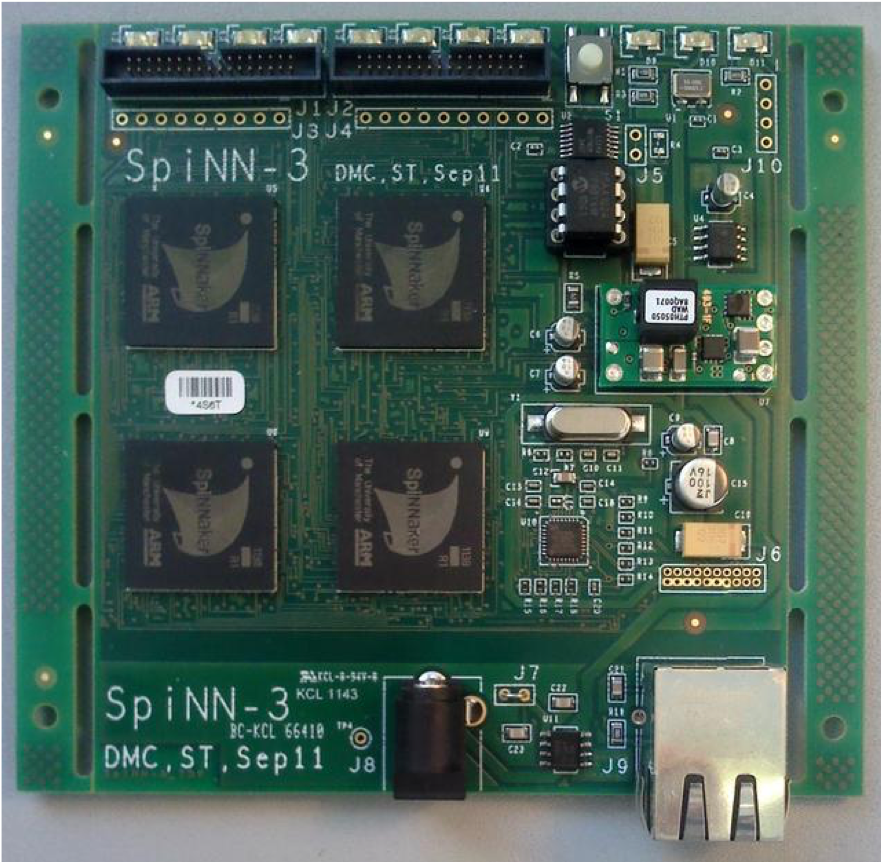
\includegraphics[width=\textwidth]{images/context/spinnaker_board.png} 
\caption{SpiNNaker board with 4 chips.}
\label{fig:spinnaker_board}
\imagesource{http://apt.cs.manchester.ac.uk/projects/SpiNNaker/hardware/index3.php}
\end{subfigure}
\begin{subfigure}{0.45\textwidth}
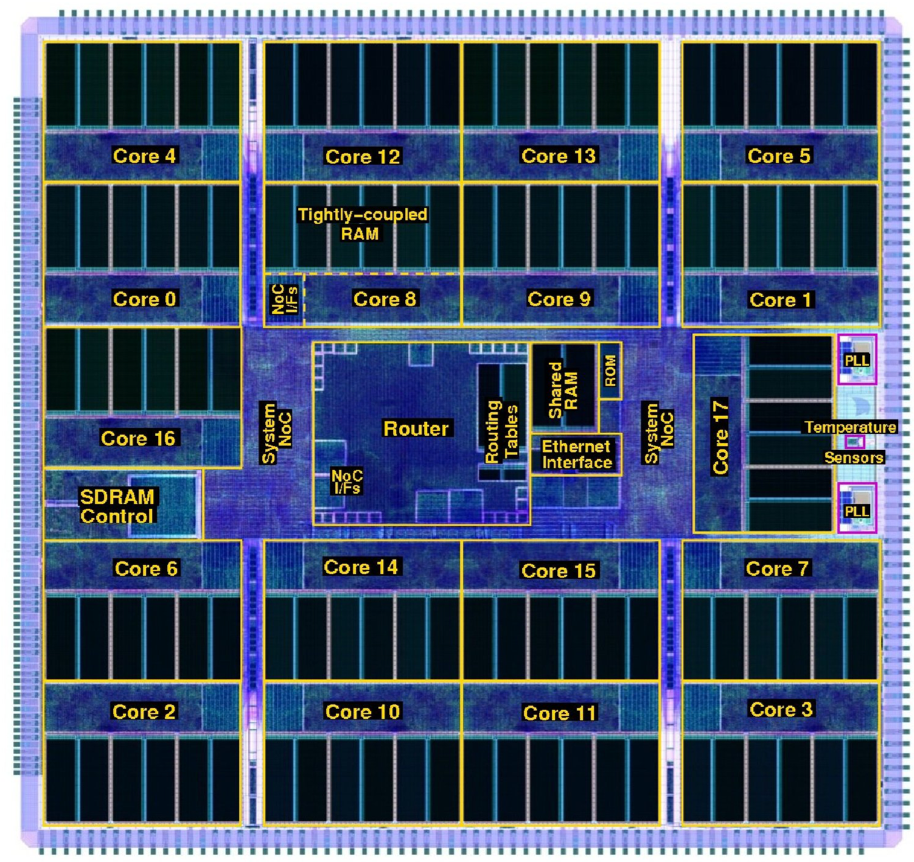
\includegraphics[width=\textwidth]{images/context/spinnaker_chip.png}
\caption{SpiNNaker chip.}
\label{fig:spinnaker_chip}
\imagesource{http://apt.cs.manchester.ac.uk/projects/SpiNNaker/SpiNNchip}
\end{subfigure}
\caption[SpiNNaker Board and Chip]{SpiNNaker board and chip}
\label{fig:spinnaker}
\end{figure}

SpiNNaker is available at different scale, from a 4 chips board shown in \cref{fig:spinnaker_board} to a 1,036,800 cores machine accessible through the Neuromorphic Computing platform of the Human Brain Project \footnote{\url{https://www.humanbrainproject.eu/en/silicon-brains/} --- Accessed 19 April 2019}.

For this project, a 4 chips board has been used. Each chip, \cref{fig:spinnaker_chip} includes 18 ARM9 cores and \SI{128}{\mega\byte} of SDRAM. The board is connected to a host machine through an Ethernet cable and it is powered through a \SI{5}{\volt} \SI{1}{\ampere} USB cable.

Each core models approximately 255 LIF neurons, for a total of about 16 thousands neuron on a 4 chips board.

\section{Dynamic Vision Sensor}
Due to the biologically inspired nature of this project and of the technologies involved, it made sense to use a Dynamic Vision Sensor as the input to the spiking neural network \cite{Hopkins2018}. 

A Dynamic Vision Sensor (DVS), also known as digital retina, is a device that records relative intensity changes for each individual pixel in continuous time. A normal frame-based camera, like the one available in a mobile phone, records entire images, the frames, a certain amount of times per second, usually 24. 

By recording only individual pixels changes, a digital retina models key properties of a biological vision system, in particular \textquote{its sparse, event-based output, its representation of relative luminance change (thus directly encoding scene reflectance change), and its rectification of positive and negative signals into separate output channels} \cite{Lichtsteiner2008}.

\begin{figure}[ht]
\centering
\captionsetup{width=0.75\linewidth}
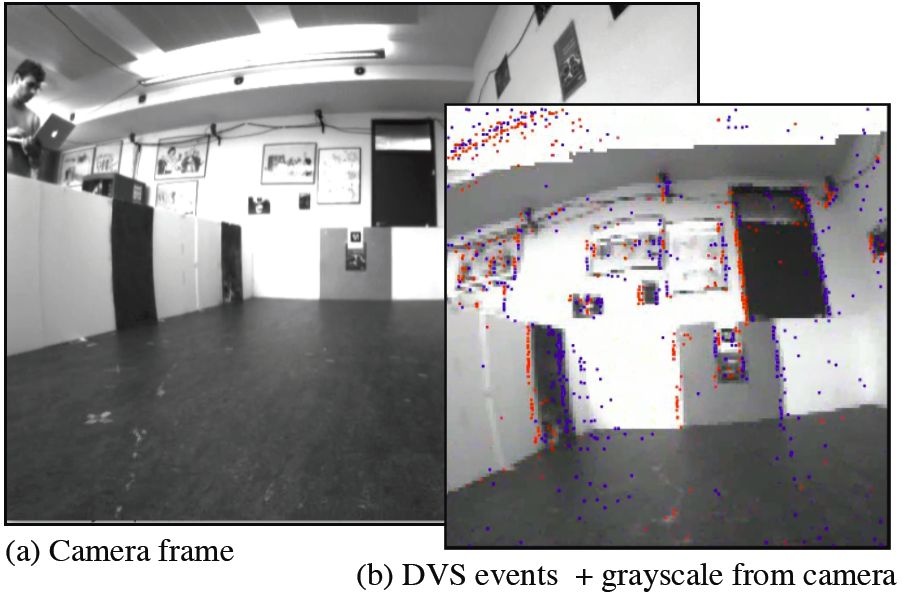
\includegraphics[scale=0.4]{images/context/dvs.jpg}
\caption[DVS comparison to frame-based device]{An example of a Dynamic Vision Sensor stream superimposed on a image from grayscale frame-based camera.}
\label{fig:dvs}
\imagesource{http://rpg.ifi.uzh.ch/research_dvs.html}
\end{figure}

Thanks to these properties, a digital retina requires low bandwidth, as it is rare that all the pixels produce a spike at the same time, has very low latency, less than \SI{1}{\milli\second}, and has a high dynamic range, higher than \SI{120}{\decibel}. On the other hand, a normal frame-based device produces a lot of redundant information since at each frame the state of all pixels is recorded, and have limited frame rates. Also, increasing the frame rate on these devices produces huge amount of data.

The digital retina output is encoded using Adress-Events Representation (AER). With this format, the only information transmitted is the $x$, $y$ position of the pixel (the address) and the time at which it spiked (the event). Two streams can be generated, one to encode positive pixel changes, and one to encode negative pixel changes. These will be called positive and negative polarities.  


\subsection{DVS Emulator}
Due to the high cost of DVS cameras, a software emulator has been developed in the School of Computer Science written in Python \cite{Garcia2017}.

\begin{figure}[ht]
\centering
\begin{subfigure}{0.49\textwidth}
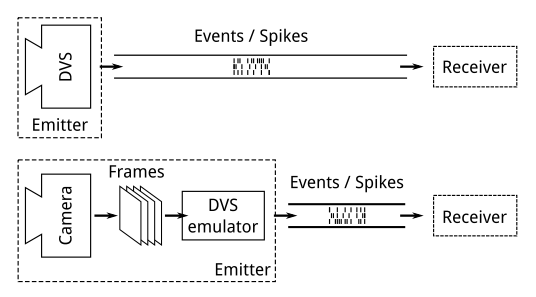
\includegraphics[width=\textwidth]{images/context/dvs_comparison.png} 
\caption{Comparison between a DVS device and the DVS emulator.}
\label{fig:dvs_comparison}
\end{subfigure}
\begin{subfigure}{0.49\textwidth}
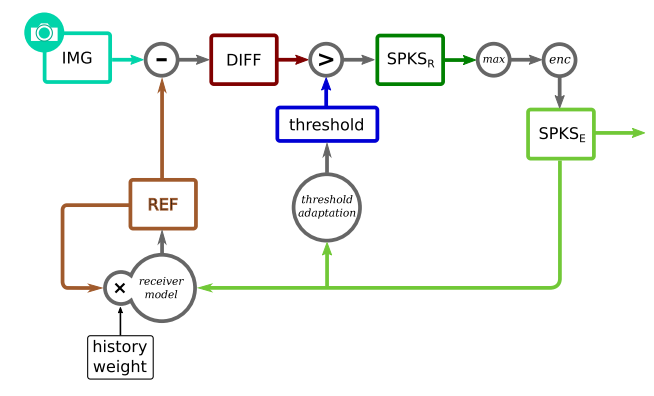
\includegraphics[width=\textwidth]{images/context/dvs_diagram.png}
\caption{Diagram of the DVS emulator and its component.}
\label{fig:dvs_diagram}
\end{subfigure}
\caption[DVS Emulator]{General overview of the DVS emulator used throughout the project. Images taken from \cite{Garcia2017}.}
\label{fig:dvs_emulator}
\end{figure}

The DVS emulator converts a frames coming from a conventional camera into a AER spike stream which can then be sent to SpiNNaker, as seen in \cref{fig:dvs_comparison}.  
\Cref{fig:dvs_diagram} shows the components of the DVS emulator. The emulator receives a frame, \textsf{IMG} in the diagram, and the differences from the previous frame are computed. The difference image goes through an adaptive threshold that adapts the per-pixel threshold based on the previous activity of the pixels: the threshold is increased if the pixels spiked previously, otherwise is reduced. The remaining pixels are considered raw spikes, $\text{\textsf{SPKS}}_\text{\textsf{R}}$ and need to be post-processed and encoded. For this project, spikes had been time encoded: the time between frames is divided into bins, each bin representing a brightness change, and a spike is sent at the time in which the pixel brightness is binned. The encoded spikes $\text{\textsf{SPKS}}_\text{\textsf{E}}$ are then used in order to update the adaptive threshold and a history decay mechanism in order to reduce errors in transmission. 
The emulator provides a lot of flexibility: the input can either be a prerecorded video or it can be used live with a webcam, and being a software artefact its behaviour can be easily changed and the results saved for reproducibility. 


\section{Motivation}
Now that an overview of the theory and technology used for this project, it makes sense to discuss the motivation behind. 

% TODO write motivation


\section{Previous Work}
There are not many application of spiking neural networks to video related tasks. The majority of them comes from the field of robotic, for example with the use of the iCub humanoid robot \cite{HernandezGarcia2018}.

Dynamic Vision Sensors had been used for several tasks in object recognition and in video related tasks, but usually the AER spike streams are processed using conventional techniques, for example clustering or other computer vision methods like Hough transform \cite{Glover2016, Glover2017}.